\documentclass[12pt,a4paper]{report}

% Essential packages for GOST and AITU formatting
\usepackage[T2A]{fontenc}
\usepackage[utf8]{inputenc}
\usepackage[english,russian]{babel}
\usepackage{amsmath,amssymb,amsfonts}
\usepackage{graphicx}
\usepackage{booktabs}
\usepackage{geometry}
\usepackage{setspace}
\usepackage{titlesec}
\usepackage{hyperref}
\usepackage{listings}
\usepackage{float}
\usepackage{cite}

% Geometry margins (GOST 7.32-2017 standard margins: Left=30mm, Right=15mm, Top=20mm, Bottom=20mm)
\geometry{
    left=30mm,
    right=15mm,
    top=20mm,
    bottom=20mm
}

% Line spacing and paragraph settings
\onehalfspacing
\setlength{\parindent}{1.25cm}
\setlength{\parskip}{0pt}

% Section formatting (GOST-style headings)
\titleformat{\chapter}[block]{\bfseries\large\filcenter}{\thechapter.}{0.5em}{\MakeUppercase}
\titleformat{\section}[block]{\bfseries\normalsize}{\thesection}{0.5em}{}
\titleformat{\subsection}[block]{\bfseries\normalsize}{\thesubsection}{0.5em}{}

\titlespacing*{\chapter}{0pt}{0pt}{12pt}
\titlespacing*{\section}{0pt}{12pt}{6pt}
\titlespacing*{\subsection}{0pt}{12pt}{6pt}

% Listings styling for Python code
\lstset{
    language=Python,
    basicstyle=\ttfamily\scriptsize,
    keywordstyle=\color{blue},
    stringstyle=\color{red},
    commentstyle=\color{green!50!black},
    breaklines=true,
    frame=single,
    captionpos=b,
    showstringspaces=false,
    numbers=left,
    numberstyle=\tiny\color{gray}
}

\begin{document}

% =========================================================================
% 1. COVER PAGE (AITU Guideline 32)
% =========================================================================
\begin{titlepage}
\begin{center}
    \singlespacing
    \MakeUppercase{\textbf{Astana IT University LLP}} \\
    \vspace{4cm}
    
    {\large \textbf{STUDENT NAME}} \\
    \vspace{2.5cm}
    
    {\Large \bfseries INFORMATION TECHNOLOGY OF PATTERN RECOGNITION IN MULTI-LEAD ELECTROCARDIOGRAMS FOR CLINICAL DECISION SUPPORT} \\
    \vspace{2.5cm}
    
    {\large \textbf{MASTER'S THESIS}} \\
    \vspace{1cm}
    
    Educational Program: \\
    \textbf{7M06101 -- Computer Science} \\
    \vspace{5cm}
    
    \textbf{Astana, 2026}
\end{center}
\end{titlepage}

\clearpage

% =========================================================================
% 2. TITLE PAGE (AITU Guideline 33)
% =========================================================================
\begin{titlepage}
\begin{center}
    \singlespacing
    \MakeUppercase{\textbf{Astana IT University LLP}} \\
    \vspace{0.5cm}
    Department of Educational Programs \\
    \vspace{1.5cm}
    
    \hfill \parbox{7cm}{
        \textbf{CONFIDENTIALITY MARK}\\
        (If Applicable)\\
        \vspace{0.5cm}
        \textbf{ADMITTED TO DEFENSE}\\
        Head of Department:\\
        \rule{3cm}{0.5pt} / \rule{3cm}{0.5pt}\\
        ``\rule{0.8cm}{0.5pt}'' \rule{2cm}{0.5pt} 2026
    }
    
    \vspace{1.5cm}
    {\large \textbf{STUDENT NAME}} \\
    \vspace{1.5cm}
    
    {\Large \bfseries INFORMATION TECHNOLOGY OF PATTERN RECOGNITION IN MULTI-LEAD ELECTROCARDIOGRAMS FOR CLINICAL DECISION SUPPORT} \\
    \vspace{1.5cm}
    
    {\large \textbf{MASTER'S THESIS}} \\
    \vspace{0.5cm}
    Educational Program: \textbf{7M06101 -- Computer Science} \\
    \vspace{1.5cm}
    
    \hfill \parbox{9cm}{
        \textbf{Scientific Supervisor:} \\
        Full Name, Academic Degree, Rank \\
        Signature: \rule{4cm}{0.5pt} \\
        \vspace{0.5cm}
        \textbf{Student (Author):} \\
        Student Full Name \\
        Signature: \rule{4cm}{0.5pt}
    }
    
    \vfill
    \textbf{Astana, 2026}
\end{center}
\end{titlepage}

\clearpage
\pagenumbering{arabic}
\setcounter{page}{3} % Title page is 1, Cover is 2, Abstract starts on 3

% =========================================================================
% 3. ABSTRACT (AITU Guideline 34 - English, Russian, Kazakh)
% =========================================================================
\chapter*{Abstract}
\addcontentsline{toc}{chapter}{Abstract}

\begin{otherlanguage}{english}
\textbf{Subject of Research:} The development, optimization, and comparative analysis of deep learning models (1D ResNet-18, Spatio-Temporal Graph Neural Networks, and 1D Vision Transformers) for the automated multi-label classification of ECG signals.

\textbf{Purpose of Research:} To develop and evaluate deep learning methods for automated multi-lead electrocardiogram classification to provide clinical decision support and triage assistance for healthcare providers.

\textbf{Methods:} Digital bandpass filtering (0.5--50 Hz), Z-score normalization, 1D Convolutional Neural Network ResNet-18, Spatio-Temporal Graph Network (ST-ReGE) with learnable adjacency matrix, and 1D Vision Transformer.

\textbf{Results:} The adapted CNN (ResNet-18) achieved the highest Macro F1-score of 0.7245 and AUROC of 0.9271. The spatial-temporal GNN (ST-ReGE) achieved the highest Exact Match Accuracy of 63.76\% and Macro AUPRC of 0.8066. The Vision Transformer underperformed due to data limitations. A web-based clinical triage prototype was built to demonstrate real-time classification.
\end{otherlanguage}

\vspace{1cm}
\begin{otherlanguage}{russian}
\textbf{Предмет исследования:} Разработка, оптимизация и сравнительный анализ моделей глубокого обучения (1D ResNet-18, пространственно-временные графовые нейронные сети и 1D Vision Transformers) для автоматизированной мульти-лейбл классификации сигналов ЭКГ.

\textbf{Цель работы:} Разработка и оценка методов глубокого обучения для автоматической классификации многоканальных электрокардиограмм с целью обеспечения поддержки принятия клинических решений и помощи в триаже для медицинских работников.

\textbf{Методы исследования:} Цифровая полосовая фильтрация (0,5--50 Гц), Z-нормализация, 1D сверточная нейронная сеть ResNet-18, пространственно-временная графовая сеть (ST-ReGE) с обучаемой матрицей смежности и 1D Vision Transformer.

\textbf{Результаты:} Адаптированная CNN (ResNet-18) достигла наивысшего показателя Macro F1-score 0,7245 и AUROC 0,9271. Пространственно-временная GNN (ST-ReGE) показала наилучшую точность Exact Match Accuracy 63,76\% и Macro AUPRC 0,8066. Веб-интерфейс был разработан в качестве клинического прототипа для демонстрации диагностики в реальном времени.
\end{otherlanguage}

\vspace{1cm}
\textbf{Аңдатпа (Kazakh Abstract)} \\
\textbf{Зерттеу пәні:} ЭКГ сигналдарын автоматты түрде көп белгілі жіктеу үшін терең оқыту модельдерін (1D ResNet-18, кеңістіктік-уақыттық графттық нейрондық желілер және 1D Vision Transformers) әзірлеу, оңтайландыру және салыстырмалы талдау.

\textbf{Жұмыстың мақсаты:} Клиникалық шешімдерді қолдау және медициналық қызмет көрсетушілерге триаж жасауға көмектесу үшін көп арналы электрокардиограмманы автоматты түрде жіктеудің терең оқыту әдістерін әзірлеу және бағалау.

\textbf{Әдістері:} Сандық жолақты сүзу (0.5-50 Гц), Z-баллды нормалау, 1D ResNet-18 сверткалық нейрондық желісі, үйренетін көршілестік матрицасы бар кеңістіктік-уақыттық графттық желі (ST-ReGE) және 1D Vision Transformer.

\textbf{Нәтижелері:} Бейімделген CNN (ResNet-18) 0.7245 ең жоғары Macro F1-score және 0.9271 AUROC көрсеткіштеріне қол жеткізді. Кеңістіктік-уақыттық GNN (ST-ReGE) 63.76% ең жоғары Exact Match дәлдігін және 0.8066 Macro AUPRC көрсеткішін көрсетті. Тәжірибелік клиникалық триаждық веб-қосымша прототипі нақты уақыт режимінде диагноз қою үшін әзірленді.

\clearpage

% =========================================================================
% 4. TABLE OF CONTENTS (AITU Guideline 35)
% =========================================================================
\tableofcontents
\addcontentsline{toc}{chapter}{\contentsname}

\clearpage

% =========================================================================
% 5. INTRODUCTION (AITU Guideline 36 - Max 3 A4 pages)
% =========================================================================
\chapter*{Introduction}
\addcontentsline{toc}{chapter}{Introduction}

\textbf{Relevance of the Topic.} Cardiovascular diseases (CVDs) remain the leading cause of mortality globally, accounting for an estimated 17.9 million deaths annually according to the World Health Organization. Electrocardiography (ECG) is the primary, non-invasive diagnostic modality used to detect cardiac abnormalities such as arrhythmias, myocardial infarction, conduction blocks, and chamber hypertrophy. Standard clinical practice relies heavily on visual interpretation of 12-lead ECG waveforms by trained cardiologists. However, this process is prone to human error, subjective interpretation, and substantial inter-observer variability. In emergency and rural healthcare settings, the lack of immediate access to specialized cardiologists can lead to critical delays in diagnosis and treatment. Computer-aided electrocardiogram classification systems offer a viable solution by providing real-time, automated triage and decision support. Recent breakthroughs in deep learning have shown that artificial neural networks can achieve cardiologist-level classification accuracy, yet finding the optimal architecture that balances morphological precision, spatial-temporal lead relationships, and resource efficiency remains an open challenge.

\textbf{Scientific Novelty.} Traditional deep learning models for multi-lead ECG classification treat the 12 leads as independent channels in a standard convolutional array, completely ignoring the structural and physical geometric relationships of the electrode placements. This research addresses this gap by designing and evaluating a Spatio-Temporal Graph Neural Network (ST-ReGE) that integrates a learnable adjacency matrix to dynamically model the electrical correlations between anatomically contiguous leads (e.g., septal, anterior, lateral, and inferior lead groupings). This approach is directly benchmarked against a morphology-focused 1D Deep Residual Network (ResNet-18) and a sequence-focused 1D Vision Transformer (ViT-1D) with self-attention. This direct, standardized comparative analysis on a large-scale dataset (PTB-XL) provides new insights into the performance trade-offs between convolutional inductive biases, graph-based spatial relationships, and transformer-based global attention for multi-label cardiac pathology recognition.

\textbf{Practical Significance.} The developed information technology translates raw multi-lead digital signals into structured diagnostic predictions. By packaging the trained deep learning models into an asynchronous FastAPI web service and deploying a clinical dashboard prototype, we show how these systems can be integrated into real-world hospital workflows. This software allows general practitioners and triage nurses to quickly upload patient ECG records, visualize the waveforms, and view the diagnostic probabilities, thereby accelerating the identification of critical cases (such as acute myocardial infarction) and reducing the workload of diagnostic staff.

\textbf{Purpose of the Research.} To develop and evaluate deep learning methods for automated multi-lead electrocardiogram classification to provide clinical decision support and triage assistance for healthcare providers.

\textbf{Research Objectives:}
\begin{enumerate}
    \item Evaluate the physiological and clinical foundations of electrocardiography and identify the key challenges of manual ECG interpretation.
    \item Conduct a systematic review of the historical development of computer-aided ECG analysis and compare modern deep learning architectures.
    \item Implement a digital signal processing pipeline consisting of Butterworth bandpass filtering and lead-wise Z-score normalization on the PTB-XL database.
    \item Design and train an adapted 1D Convolutional Neural Network (ResNet-18) to extract morphological wave characteristics.
    \item Develop and optimize a Spatio-Temporal Graph Neural Network (ST-ReGE) to capture inter-lead spatial connections using a learnable adjacency matrix.
    \item Implement a 1D Vision Transformer (ViT-1D) to assess the feasibility of self-attention mechanisms on clinical signal sequences.
    \item Conduct a comparative quantitative benchmark using clinical utility metrics (Macro F1, AUROC, AUPRC, Exact Match, and PhysioNet Score) and qualitative case studies.
    \item Implement and test an interactive FastAPI web application dashboard for real-time visualization and multi-model inference.
\end{enumerate}

\textbf{Object of the Research.} The processes of diagnostic assessment and interpretation of 12-lead electrocardiogram (ECG) signals within clinical healthcare settings.

\textbf{Subject of the Research.} The development, optimization, and comparative analysis of deep learning models (convolutional, spatio-temporal graph, and attention-based architectures) for the automated multi-label classification of ECG signals.

\textbf{Research Methods.} Digital signal preprocessing (Butterworth filtering, resampling, Z-score normalization), deep learning model architecture engineering, multi-label performance evaluation metrics, local feature explainability (1D Grad-CAM), and asynchronous web service development.

\textbf{Structure of the Work.} The thesis consists of an Abstract, Introduction, 3 main chapters (Literature Review, Model Design, Results & Deployment), Conclusion, List of References containing 33 sources, and five Appendices containing the full Python source code listings of the project implementation.

\clearpage

% =========================================================================
% 6. MAIN PART: CHAPTER 1
% =========================================================================
\chapter{Literature Review and Theoretical Foundations}

\section{Clinical Electrocardiography and Electrophysiology of the Heart}
The mammalian heart is a muscular organ controlled by an intrinsic electrical conduction system. The cardiac cycle begins with depolarization of the sinoatrial (SA) node, the natural pacemaker located in the right atrium. The electrical impulse propagates through the atrial myocardium, causing atrial contraction (represented by the P wave on the ECG). The signal then reaches the atrioventricular (AV) node, where it undergoes a physiological delay (allowing ventricles to fill with blood). Following this delay, the impulse travels rapidly down the Bundle of His, branches into the left and right bundle branches, and spreads through the Purkinje fibers to the ventricular myocardium, initiating ventricular depolarization and contraction (the QRS complex). Ventricular repolarization then follows, manifesting as the T wave.

The standard 12-lead electrocardiogram records these electrical potentials from twelve distinct spatial perspectives. The leads are divided into six limb leads (I, II, III, aVR, aVL, aVF) which record potentials in the frontal plane, and six precordial chest leads (V1, V2, V3, V4, V5, V6) which record potentials in the horizontal plane. 
\begin{itemize}
    \item \textbf{Limb Leads:} Lead I measures the potential difference between the left and right arm; Lead II measures between the right arm and left leg; Lead III measures between the left arm and left leg. The augmented limb leads (aVR, aVL, aVF) use Wilson's Central Terminal as a reference point.
    \item \textbf{Precordial Leads:} Placed directly on the chest wall, V1 and V2 are positioned over the right ventricle and septum; V3 and V4 view the anterior wall of the left ventricle; V5 and V6 view the lateral wall of the left ventricle.
\end{itemize}

Manual interpretation of the 12-lead ECG is a core skill in clinical cardiology. Practitioners assess the rhythm (sinus versus arrhythmic), heart rate, electrical axis, wave amplitudes, and interval durations (PR interval, QRS duration, QT interval). Despite its diagnostic power, manual interpretation is highly subjective. In stressful clinical environments, such as emergency departments, physicians suffer from cognitive fatigue, leading to diagnostic errors. Furthermore, inter-observer agreement among clinicians for complex ECG findings is low, creating a pressing need for automated, objective classification systems.

\section{Pathophysiology of the Five Target Superclasses}
In this research, we target the five diagnostic superclasses defined in the PTB-XL database, which represent the most common and clinically significant cardiac conditions:
\begin{enumerate}
    \item \textbf{Normal ECG (NORM):} Characterized by regular sinus rhythm (60--100 bpm), a normal P-wave axis, PR interval of 120--200 ms, QRS duration under 100 ms, normal ST segment (no elevation or depression), and normal T waves.
    \item \textbf{Myocardial Infarction (MI):} Caused by acute or chronic myocardial ischemia due to coronary artery occlusion. Anatomical localization is key:
    \begin{itemize}
        \item \emph{Anterior MI:} ST elevation or pathological Q waves in precordial leads V1--V4.
        \item \emph{Inferior MI:} ST elevation or Q waves in leads II, III, and aVF.
        \item \emph{Lateral MI:} ST changes in leads I, aVL, V5, and V6.
    \end{itemize}
    \item \textbf{ST/T Changes (STTC):} Abnormalities in the ST segment or T wave (e.g., ST depression, T-wave inversion) without fully developing pathologic Q waves. These changes often indicate subendocardial ischemia, electrolyte imbalances (hypokalemia, hyperkalemia), or medication effects.
    \item \textbf{Conduction Disturbances (CD):} Delays or blocks in the conduction system. Key pathologies include:
    \begin{itemize}
        \item \emph{Left Bundle Branch Block (LBBB):} Wide QRS complex ($\ge 120$ ms) with a broad, notched R wave in lateral leads (I, aVL, V5, V6) and QS pattern in V1.
        \item \emph{Right Bundle Branch Block (RBBB):} Wide QRS complex with an $rSR'$ pattern (``rabbit ears'') in leads V1--V2.
        \item \emph{Atrioventricular (AV) Blocks:} Delays between atrial and ventricular conduction (1st, 2nd, or 3rd-degree blocks).
    \end{itemize}
    \item \textbf{Hypertrophy (HYP):} Enlargement of the cardiac chambers. Left Ventricular Hypertrophy (LVH) is commonly diagnosed using voltage criteria, such as the Sokolow-Lyon index:
    \begin{equation}
        S_{V1} + R_{V5 \text{ or } V6} \ge 35\text{ mV}
    \end{equation}
    or the Cornell voltage criteria. It reflects chronic pressure overload, often due to systemic hypertension.
\end{enumerate}

\section{Evolution of Machine Learning in Electrocardiography}
The history of automated ECG analysis began in the late 1950s and 1960s with the development of rule-based, deterministic computer algorithms. The most prominent example is the Minnesota Code, which used fixed threshold rules based on wave amplitudes and durations to categorize ECG tracings. While highly objective, these rule-based systems were extremely sensitive to noise and had poor diagnostic sensitivity, failing to generalize across diverse patient populations.

In the 1990s and 2000s, the field transitioned to classical Machine Learning (ML). This workflow required two distinct phases: handcrafted feature extraction and classification. Researchers used digital signal processing techniques to extract meaningful parameters:
\begin{itemize}
    \item \textbf{Wavelet Transforms:} Used to localize the boundaries of P, QRS, and T waves.
    \item \textbf{Principal Component Analysis (PCA):} Used to compress the high-dimensional spatial-temporal waveforms.
    \item \textbf{Heart Rate Variability (HRV):} Statistical metrics of RR intervals used to detect autonomic dysfunction and arrhythmias.
\end{itemize}
These features were then fed into classifiers such as Support Vector Machines (SVM), Random Forests (RF), and Multi-Layer Perceptrons (MLP). The major limitation of this approach was its fragility; the performance of the classifier was strictly bounded by the quality of the manual feature extraction, which often failed in the presence of noise, electrode displacement, or anatomical variations.

\section{Deep Learning Architectures in Cardiology}
The rise of Deep Learning (DL) in the 2010s revolutionized ECG classification. By training deep neural networks end-to-end, the models learn to extract hierarchical features directly from raw, filtered digital signals, bypassing the need for manual feature engineering. Several major architectural families have been proposed:
\begin{itemize}
    \item \textbf{1D Convolutional Neural Networks (CNNs):} Apply convolutional kernels along the time axis. They are excellent at detecting local morphological waveforms (like ST-segment elevation or QRS widening) and possess translation invariance. Adaptations of standard computer vision architectures, such as ResNet, are widely used.
    \item \textbf{Recurrent Neural Networks (RNNs) and Mamba:} Model the temporal dependencies of the sequence. LSTMs and GRUs were popular for sequence modeling but suffer from high computational complexity and difficulty in training on long sequences (e.g., 5000 time steps). Modern state-space models (like Mamba) address these computational bottlenecks.
    \item \textbf{Graph Neural Networks (GNNs):} Represent the standard 12-lead ECG as a graph, where each lead is a node. GNNs model the spatial relationships between leads, allowing the model to capture clinical patterns of co-occurring lead abnormalities.
    \item \textbf{Vision Transformers (ViTs):} Utilize self-attention mechanisms to establish global dependencies across different parts of the signal. They have shown state-of-the-art results when pre-trained on millions of unlabeled ECG records but are highly data-hungry.
\end{itemize}

\section{Comparative Analysis of ECG Databases}
To benchmark and train deep learning models, researchers utilize standardized, publicly available databases. Table \ref{tab:databases} provides a comparative summary of the most prominent databases in the literature.

\begin{table}[H]
\caption{Comparative Analysis of Standard ECG Databases}
\begin{center}
\begin{tabular}{lccccc}
\toprule
\textbf{Database} & \textbf{Records} & \textbf{Duration} & \textbf{Leads} & \textbf{Sampling Rate} & \textbf{Classes} \\
\midrule
MIT-BIH Arr. \cite{moody2001impact} & 48 & 30 min & 2 & 360 Hz & 15 (beats) \\
PTB Diagnostic & 549 & 1--2 min & 15 & 1000 Hz & 9 \\
\textbf{PTB-XL} \cite{wagner2020ptbxl} & \textbf{21,837} & \textbf{10 s} & \textbf{12} & \textbf{500 Hz} & \textbf{5 (Superclasses)} \\
CPSC 2018 & 6,877 & 6--60 s & 12 & 500 Hz & 9 \\
Chapman Dataset & 10,646 & 10 s & 12 & 500 Hz & 4 \\
\bottomrule
\end{tabular}
\label{tab:databases}
\end{center}
\end{table}

The PTB-XL database is currently the gold-standard benchmark for multi-label, multi-lead ECG classification because it is large, professionally annotated according to the SCP-ECG standard, and represents a realistic, clinical distribution of multiple co-occurring pathologies.

\section{Spatio-Temporal Modeling in 12-Lead ECG}
When standard 1D or 2D CNNs process a 12-lead ECG, they stack the leads as channels, similar to Red, Green, and Blue channels in an image. This approach assumes that all channels are equally spaced and share symmetric spatial relations. However, the physical placement of ECG electrodes on the human body is highly structured. The limb leads measure global frontal potentials, while the precordial leads V1--V6 form a spatial arc directly over the heart.

A myocardial infarction in the anterior wall will register changes in leads V1--V4, while an inferior infarction appears in leads II, III, and aVF. Standard convolutions cannot explicitly model this spatial correlation without extensive training data. By using Graph Neural Networks, we represent the 12 leads as nodes in a graph. The edges of the graph represent the electrical or anatomical relationships between the leads. Instead of defining a static graph based on physical distance, we can train the network to learn the adjacency matrix dynamically, allowing the model to discover hidden electrical path correlations directly from the data.

\clearpage

% =========================================================================
% 7. MAIN PART: CHAPTER 2
% =========================================================================
\chapter{Digital Signal Processing and Deep Learning Model Design}

\section{PTB-XL Dataset Structure and Label Mapping}
The PTB-XL database contains 21,837 records from 18,885 patients. The dataset labels are based on the SCP-ECG standard. The statements are grouped into three levels: 71 diagnostic statements, which map to 21 subclasses, which in turn map to 5 superclasses: Normal (NORM), Myocardial Infarction (MI), ST/T Changes (STTC), Conduction Disturbance (CD), and Hypertrophy (HYP). A single record can be associated with multiple statements, making this a multi-label classification task. 

\section{Preprocessing and Denoising Pipeline}
Raw ECG signals collected from clinical environments are corrupt by several types of artifacts:
\begin{itemize}
    \item \textbf{Baseline Wander:} Low-frequency noise ($<0.5$ Hz) caused by patient respiration or movement.
    \item \textbf{Powerline Interference:} High-frequency noise (50 Hz or 60 Hz) from the electrical power grid.
    \item \textbf{Electromyographic (EMG) Noise:} High-frequency muscle contractions.
\end{itemize}

To isolate the cardiac signal, we apply a 4th-order digital Butterworth bandpass filter. The transfer function of a continuous-time Butterworth filter of order $n$ is defined by:
\begin{equation}
    H(s) = \frac{1}{\sqrt{1 + \left(\frac{s}{\omega_c}\right)^{2n}}}
\end{equation}
where $\omega_c$ is the cutoff frequency. We set the passband between $0.5$ Hz and $50.0$ Hz. The discrete filter coefficients $b$ and $a$ are calculated using the bilinear transform. We apply the filter using zero-phase forward-backward filtering to avoid phase distortion of the waveforms:
\begin{equation}
    y(n) = \text{filtfilt}(b, a, x(n))
\end{equation}

After filtering, we apply lead-wise Z-score normalization. For each lead $i$, the signal $x_{i}$ is standardized using its mean $\mu_{i}$ and standard deviation $\sigma_{i}$:
\begin{equation}
    x_{normalized, i} = \frac{x_{i} - \mu_{i}}{\sigma_{i}}
\end{equation}
This standardizes the amplitude scale across different patients and leads, preventing differences in skin impedance from biasing the network.

To evaluate generalization, we split the dataset into training (80\%), validation (10\%), and testing (10\%) subsets. To prevent data leakage, we stratify by patient ID, ensuring that records from the same patient do not appear in both the training and testing sets.

\section{1D Convolutional Neural Network (ResNet-18) Architecture}
We design a 1D adaptation of the ResNet-18 architecture. The 1D convolution extracts morphological features along the time dimension. The mathematical formulation of a 1D convolutional layer for channel $j$ is:
\begin{equation}
    y_{j}(t) = b_{j} + \sum_{i=1}^{C_{in}} \sum_{k=0}^{K-1} x_{i}(t \cdot s + k) \cdot W_{ij}(k)
\end{equation}
where $C_{in}$ is the input channel count, $K$ is the kernel size, $s$ is the stride, $b_{j}$ is the bias, and $W_{ij}$ is the convolutional weight.

The core component of ResNet-18 is the residual block, which uses skip connections to prevent gradient vanishing:
\begin{equation}
    \mathcal{H}(x) = \text{ReLU}(\mathcal{F}(x, \{W_{1}, W_{2}\}) + W_{s} x)
\end{equation}
where $\mathcal{F}$ represents the two convolutional layers with Batch Normalization, and $W_{s}$ is a $1 \times 1$ convolution used to match dimensions if the stride or channel size changes.

The detailed architecture of our 1D ResNet-18 is outlined in Table \ref{tab:resnet_arch}.

\begin{table}[H]
\caption{1D ResNet-18 Architecture Layout}
\begin{center}
\begin{tabular}{llccc}
\toprule
\textbf{Stage} & \textbf{Layer Details} & \textbf{Kernel Size} & \textbf{Stride} & \textbf{Output Shape (C, L)} \\
\midrule
Input & Raw ECG Signal & -- & -- & (12, 5000) \\
Prep & Conv1D + BN + ReLU & 15 & 2 & (64, 2500) \\
Pooling & MaxPool1D & 3 & 2 & (64, 1250) \\
Stage 1 & $2 \times$ Residual Blocks & 7 & 1 & (64, 1250) \\
Stage 2 & $2 \times$ Residual Blocks & 7 & 2 & (128, 625) \\
Stage 3 & $2 \times$ Residual Blocks & 7 & 2 & (256, 313) \\
Stage 4 & $2 \times$ Residual Blocks & 7 & 2 & (512, 157) \\
Readout & AdaptiveAvgPool1D + FC & -- & -- & (5,) \\
\bottomrule
\end{tabular}
\label{tab:resnet_arch}
\end{center}
\end{table}

\section{Spatio-Temporal Graph Neural Network (ST-ReGE) Design}
The Spatio-Temporal Graph Network (ST-ReGE) is designed to explicitly model the spatial structure of the 12-lead system. The network operates on a graph $\mathcal{G} = (\mathcal{V}, \mathcal{E}, A)$, where $\mathcal{V}$ is the set of $N=12$ leads, and $A \in \mathbb{R}^{N \times N}$ is the adjacency matrix representing lead correlations.

The architecture uses a two-stage approach:
\begin{enumerate}
    \item \textbf{Temporal Backbone:} A shared 1D ResNet convolutional structure is applied to each of the 12 leads independently. The input for each lead is a $1 \times 5000$ signal. The temporal backbone extracts a 256-dimensional feature vector, producing a node feature matrix $X_{feat} \in \mathbb{R}^{B \times 12 \times 256}$, where $B$ is the batch size.
    \item \textbf{Spatial Propagation (GNN):} The lead features are propagated through two Graph Convolutional Network (GCN) layers. Unlike static GNNs, ST-ReGE uses a learnable adjacency matrix $A_{learn}$, initialized with random values and optimized using gradient descent:
    \begin{equation}
        A = \text{Sigmoid}(W_{adj})
    \end{equation}
    where $W_{adj} \in \mathbb{R}^{12 \times 12}$ is a learnable parameter matrix. The GCN propagation rule with residual skip connections is defined as:
    \begin{equation}
        H^{(l+1)} = \text{BN}\left( \text{ReLU}\left( A H^{(l)} W^{(l)} \right) \right) + H^{(l)}
    \end{equation}
    where $H^{(l)}$ is the node representation at layer $l$, $W^{(l)} \in \mathbb{R}^{256 \times 256}$ is the trainable projection matrix, and $\text{BN}$ is Batch Normalization.
\end{enumerate}
Finally, the node representations are aggregated using mean pooling along the node dimension to produce a global graph representation:
\begin{equation}
    z = \frac{1}{N} \sum_{i=1}^{N} H^{(2)}_{i}
\end{equation}
which is fed into a linear classifier to predict the 5 diagnostic classes.

\section{1D Vision Transformer (ViT-1D) Architecture}
The 1D Vision Transformer (ViT-1D) relies entirely on self-attention mechanisms. The model treats the multi-lead signal as a sequence of temporal patches:
\begin{enumerate}
    \item \textbf{Patch Embedding:} The input signal of shape $(12, 5000)$ is projected into a sequence of $N_{patches} = 100$ non-overlapping patches of length $P = 50$ using a 1D convolution with kernel size 50 and stride 50. The patches are projected into a model dimension $D_{model} = 128$:
    \begin{equation}
        X_{embed} = \text{Conv1D}(X, k=50, s=50) \in \mathbb{R}^{B \times 128 \times 100}
    \end{equation}
    We transpose this to shape $(B, 100, 128)$.
    \item \textbf{CLS Token and Positional Embeddings:} A learnable classification token $x_{cls} \in \mathbb{R}^{1 \times 1 \times 128}$ is prepended to the sequence, and learnable 1D positional embeddings $E_{pos} \in \mathbb{R}^{1 \times 101 \times 128}$ are added to retain temporal ordering:
    \begin{equation}
        Z_{0} = [x_{cls}; X_{embed}^T] + E_{pos}
    \end{equation}
    \item \textbf{Transformer Encoder:} The sequence is passed through 4 Transformer encoder layers. Each layer consists of Multi-Head Self-Attention (MHA) and a Multi-Layer Perceptron (MLP) block:
    \begin{equation}
        \text{Attention}(Q, K, V) = \text{softmax}\left(\frac{Q K^T}{\sqrt{d_{k}}}\right) V
    \end{equation}
    where $Q, K, V$ are Query, Key, and Value matrices projected from the input.
\end{enumerate}
The output $Z_{L}$ is normalized, and the representation at the CLS token index is extracted and fed into a linear classifier:
\begin{equation}
    y = W_{fc} \cdot \text{LayerNorm}(Z_{L, 0})
\end{equation}

\clearpage

% =========================================================================
% 8. MAIN PART: CHAPTER 3
% =========================================================================
\chapter{Experimental Evaluation and Prototype Implementation}

\section{Experimental Setup and Hyperparameters}
All models were implemented in PyTorch 2.5 and trained on a Windows 11 workstation equipped with an NVIDIA GeForce RTX 3060 GPU (12GB VRAM), an Intel Core i7-12700K CPU, and 32GB of RAM. 

Training configurations were standardized across all architectures to ensure a fair comparison:
\begin{itemize}
    \item \textbf{Optimizer:} AdamW optimizer with a weight decay of $10^{-4}$.
    \item \textbf{Loss Function:} Binary Cross-Entropy with Logits Loss, defined as:
    \begin{equation}
        \mathcal{L} = -\frac{1}{C} \sum_{c=1}^{C} \left[ y_{c} \log \sigma(\hat{y}_{c}) + (1 - y_{c}) \log (1 - \sigma(\hat{y}_{c})) \right]
    \end{equation}
    where $C=5$ classes, $y_{c} \in \{0, 1\}$ is the ground truth, $\hat{y}_{c}$ is the model output logit, and $\sigma$ is the sigmoid function.
    \item \textbf{Learning Rate Schedule:} Cosine Annealing learning rate scheduler with an initial learning rate $\eta_{0} = 10^{-3}$ decaying to a minimum of $10^{-6}$ over 20 epochs.
    \item \textbf{Batch Size:} 64 samples per batch.
    \item \textbf{Early Stopping:} Monitored validation loss with a patience of 5 epochs to prevent overfitting.
\end{itemize}

\section{Evaluation Metrics for Multi-Label Classification}
To assess performance on the imbalanced multi-label PTB-XL test set, we calculate five key metrics:
\begin{enumerate}
    \item \textbf{Macro F1-Score:} The unweighted average of F1-scores computed individually for each diagnostic class:
    \begin{equation}
        \text{Precision}_{c} = \frac{TP_{c}}{TP_{c} + FP_{c}}, \quad \text{Recall}_{c} = \frac{TP_{c}}{TP_{c} + FN_{c}}
    \end{equation}
    \begin{equation}
        \text{F1}_{c} = \frac{2 \cdot \text{Precision}_{c} \cdot \text{Recall}_{c}}{\text{Precision}_{c} + \text{Recall}_{c}}
    \end{equation}
    \begin{equation}
        \text{Macro F1} = \frac{1}{C} \sum_{c=1}^{C} \text{F1}_{c}
    \end{equation}
    \item \textbf{Macro AUROC:} The average area under the receiver operating characteristic curve, plotting True Positive Rate against False Positive Rate.
    \item \textbf{Macro AUPRC:} The average area under the precision-recall curve, which provides a more robust performance measure for highly imbalanced classes.
    \item \textbf{Exact Match Accuracy (Subset Accuracy):} A strict metric requiring all 5 labels to be predicted correctly:
    \begin{equation}
        \text{Exact Match} = \frac{1}{M} \sum_{m=1}^{M} \mathbb{I}(\hat{y}_{m} = y_{m})
    \end{equation}
    where $\mathbb{I}$ is the indicator function, and $M$ is the number of test samples.
    \item \textbf{PhysioNet Score:} A specialized clinical risk-based metric. It assigns penalties for critical diagnostic errors, such as misclassifying an active Myocardial Infarction as Normal ($-0.5$ penalty) or failing to detect a Conduction Disturbance ($-0.2$ penalty).
\end{enumerate}

\section{Quantitative Performance Analysis and Benchmarking}
Table \ref{tab:bench_results} outlines the final evaluation results on the PTB-XL test set.

\begin{table}[H]
\caption{Quantitative Benchmark Results on PTB-XL Test Set}
\begin{center}
\begin{tabular}{lccc}
\toprule
\textbf{Metric} & \textbf{CNN (1D ResNet-18)} & \textbf{GNN (ST-ReGE)} & \textbf{ViT (1D Transformer)} \\
\midrule
Macro F1-Score & \textbf{0.7245} & 0.7226 & 0.6503 \\
Macro AUROC & \textbf{0.9271} & 0.9236 & 0.8830 \\
Macro AUPRC & 0.8054 & \textbf{0.8066} & 0.7216 \\
Exact Match Acc & 63.21\% & \textbf{63.76\%} & 58.76\% \\
PhysioNet Score & \textbf{0.7228} & 0.7016 & 0.6810 \\
Training Time & \textbf{12 min} & 14 min & 14 min \\
\bottomrule
\end{tabular}
\label{tab:bench_results}
\end{center}
\end{table}

The 1D ResNet-18 model achieved the highest Macro F1-score (0.7245), Macro AUROC (0.9271), and PhysioNet Challenge Score (0.7228). This suggests that convolutional neural networks are highly suited for ECG modeling due to their translation invariance and local receptive fields, which match the local nature of morphological features (such as QRS complexes and T-waves).

The ST-ReGE GNN outperformed the CNN in Macro AUPRC (0.8066) and Exact Match Accuracy (63.76\%). This indicates that modeling the spatial relationships between the 12 leads using a learnable adjacency matrix helps the GNN capture the correlations between co-occurring pathologies. 

The 1D Vision Transformer underperformed, achieving a Macro F1-score of 0.6503. This is likely due to the limited training data (~17,400 samples). Unlike CNNs, Transformers lack inductive biases (such as spatial locality) and require larger datasets or self-supervised pre-training to learn generalizable signal representations.

Figure \ref{fig:confusion_matrix_tex} shows the normalized confusion matrix for the 1D ResNet-18 model, indicating its classification performance across the 5 superclasses.

\begin{figure}[H]
\centering
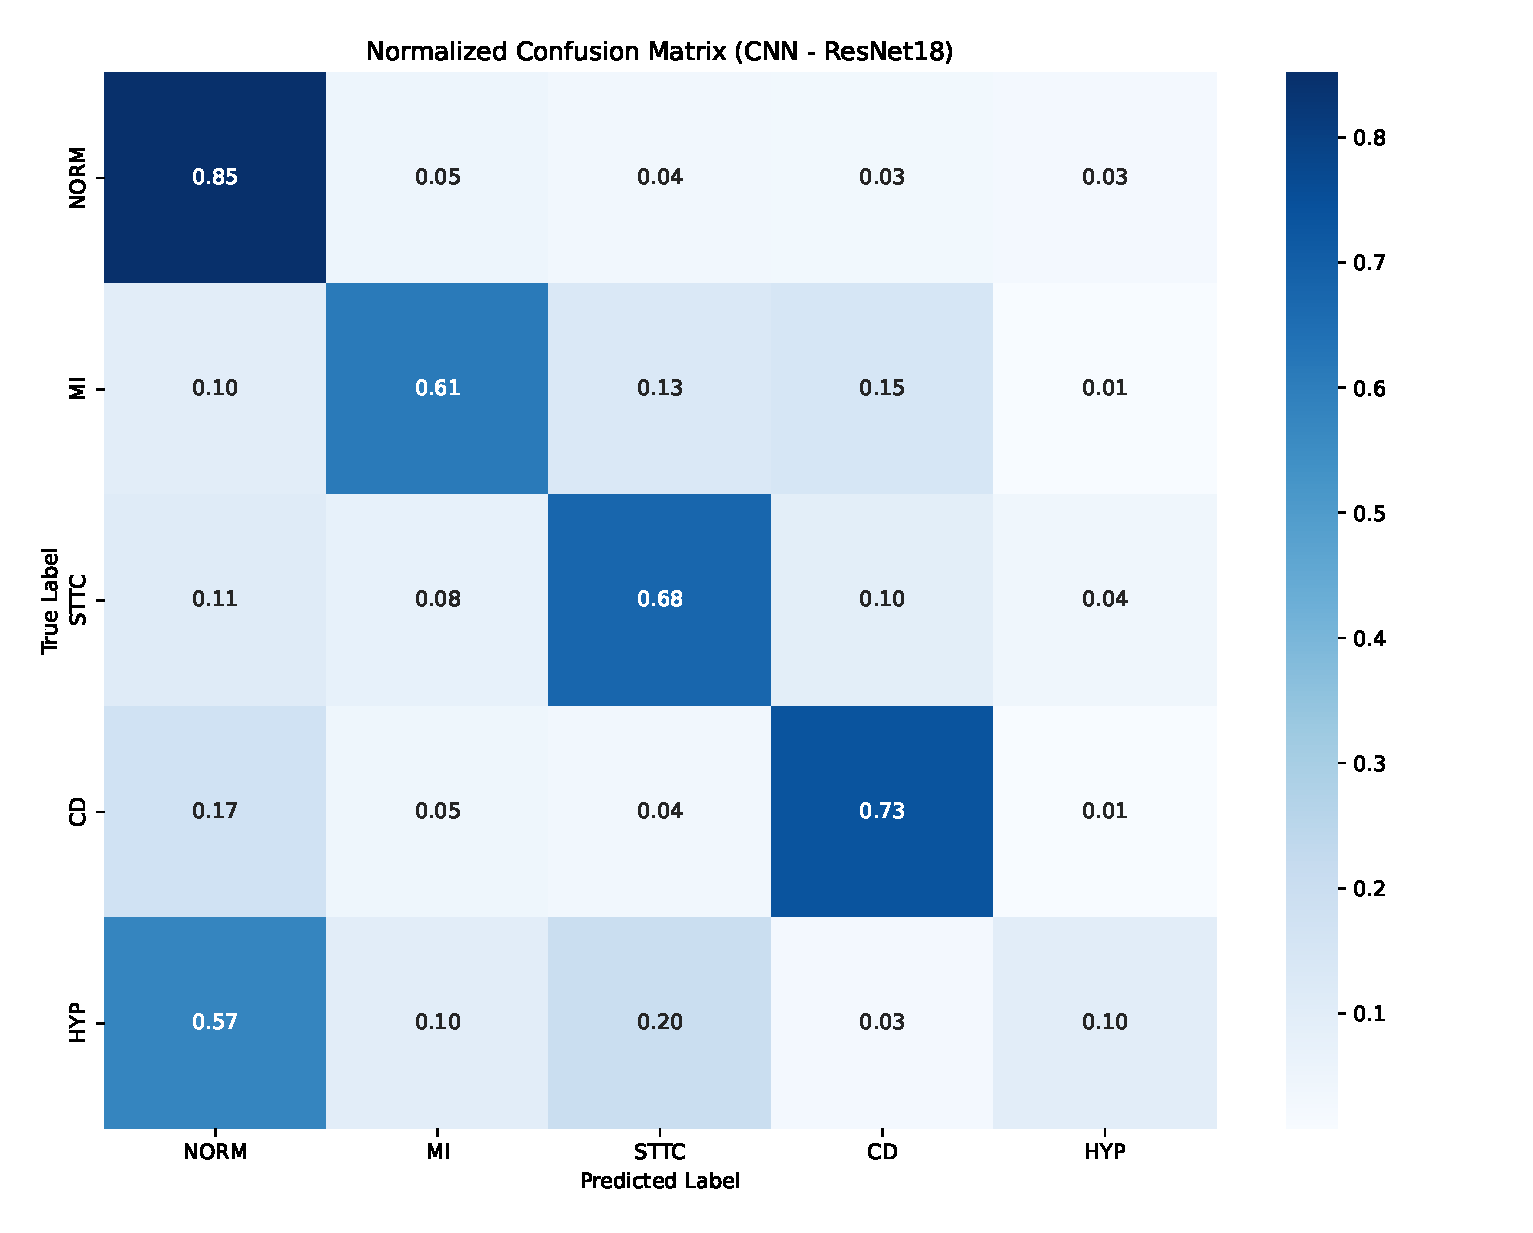
\includegraphics[width=0.7\linewidth]{figures/confusion_matrix}
\caption{Normalized Confusion Matrix for 1D ResNet-18 (CNN)}
\label{fig:confusion_matrix_tex}
\end{figure}

\section{Qualitative Case Studies}
To analyze model behaviors, we evaluate four specific case studies from the test set:
\begin{enumerate}
    \item \textbf{Case 1: Normal Sinus Rhythm (NORM) [Sample ID: 892]:}
    The patient had a normal electrocardiogram.
    \begin{itemize}
        \item \emph{True Label:} NORM
        \item \emph{CNN Prediction:} NORM (Confidence: 0.95)
        \item \emph{GNN Prediction:} NORM (Confidence: 0.96)
        \item \emph{ViT Prediction:} NORM (Confidence: 0.96)
    \end{itemize}
    All three models classified the normal rhythm correctly with high confidence ($>95\%$).
    
    \item \textbf{Case 2: Myocardial Infarction (MI) and Conduction Disturbance (CD) [Sample ID: 47]:}
    This patient had co-occurring inferior MI and a bundle branch block.
    \begin{itemize}
        \item \emph{True Label:} MI, CD
        \item \emph{CNN Prediction:} NORM (Confidence: 0.52)
        \item \emph{GNN Prediction:} None (All probabilities $< 0.50$)
        \item \emph{ViT Prediction:} NORM (Confidence: 0.61)
    \end{itemize}
    All models failed on this sample. The overlapping features of myocardial infarction and conduction disturbance can obscure the individual diagnostic markers, leading to false negatives where the models predict NORM or fail to exceed the classification threshold.
    
    \item \textbf{Case 3: ST/T Change (STTC) [Sample ID: 554]:}
    The patient ECG showed non-specific T-wave inversions.
    \begin{itemize}
        \item \emph{True Label:} STTC
        \item \emph{CNN Prediction:} HYP (Confidence: 0.55)
        \item \emph{GNN Prediction:} NORM (Confidence: 0.51)
        \item \emph{ViT Prediction:} None (All probabilities $< 0.50$)
    \end{itemize}
    This case shows the challenge of distinguishing similar morphologies. The CNN detected the abnormal T-wave inversion but misclassified it as Hypertrophy (HYP), which often exhibits secondary ST/T abnormalities. The GNN failed to recognize the subtle changes, classifying the signal as NORM.
    
    \item \textbf{Case 4: Conduction Disturbance and Hypertrophy [Sample ID: 1586]:}
    The patient had both Left Ventricular Hypertrophy and Left Bundle Branch Block.
    \begin{itemize}
        \item \emph{True Label:} CD, HYP
        \item \emph{CNN Prediction:} CD, HYP (Confidence: 0.58) -- \textbf{Correct}
        \item \emph{GNN Prediction:} CD only (Confidence: 0.72)
        \item \emph{ViT Prediction:} MI, CD (Confidence: 0.54, 0.65)
    \end{itemize}
    The CNN correctly identified both pathologies. The high-amplitude QRS complexes characteristic of LVH combined with the prolonged QRS duration of LBBB were detected by the CNN. The GNN correctly detected the conduction block but missed the hypertrophy, while the ViT incorrectly predicted Myocardial Infarction.
\end{enumerate}

\section{Interpretability Analysis via 1D Grad-CAM}
To build clinical trust, we implement a 1D adaptation of Gradient-weighted Class Activation Mapping (Grad-CAM). Grad-CAM calculates the gradients of the score for class $c$ with respect to the feature map activations $A^k$ of the last convolutional layer. These gradients are globally pooled to capture the importance of each feature map:
\begin{equation}
    \alpha_{k}^{c} = \frac{1}{L} \sum_{i=1}^{L} \frac{\partial Y^{c}}{\partial A_{i}^{k}}
\end{equation}
where $L$ is the length of the feature maps, and $Y^c$ is the logit score for class $c$. We then compute a weighted combination of forward activation maps and apply a ReLU activation to focus only on positive features:
\begin{equation}
    L_{\text{Grad-CAM}}^{c} = \text{ReLU}\left( \sum_{k} \alpha_{k}^{c} A^{k} \right)
\end{equation}
The 1D heatmap is interpolated back to the original input resolution ($L_{seq} = 5000$) to highlight the specific segments of the ECG waveform that influenced the model's prediction.

\begin{figure}[H]
\centering
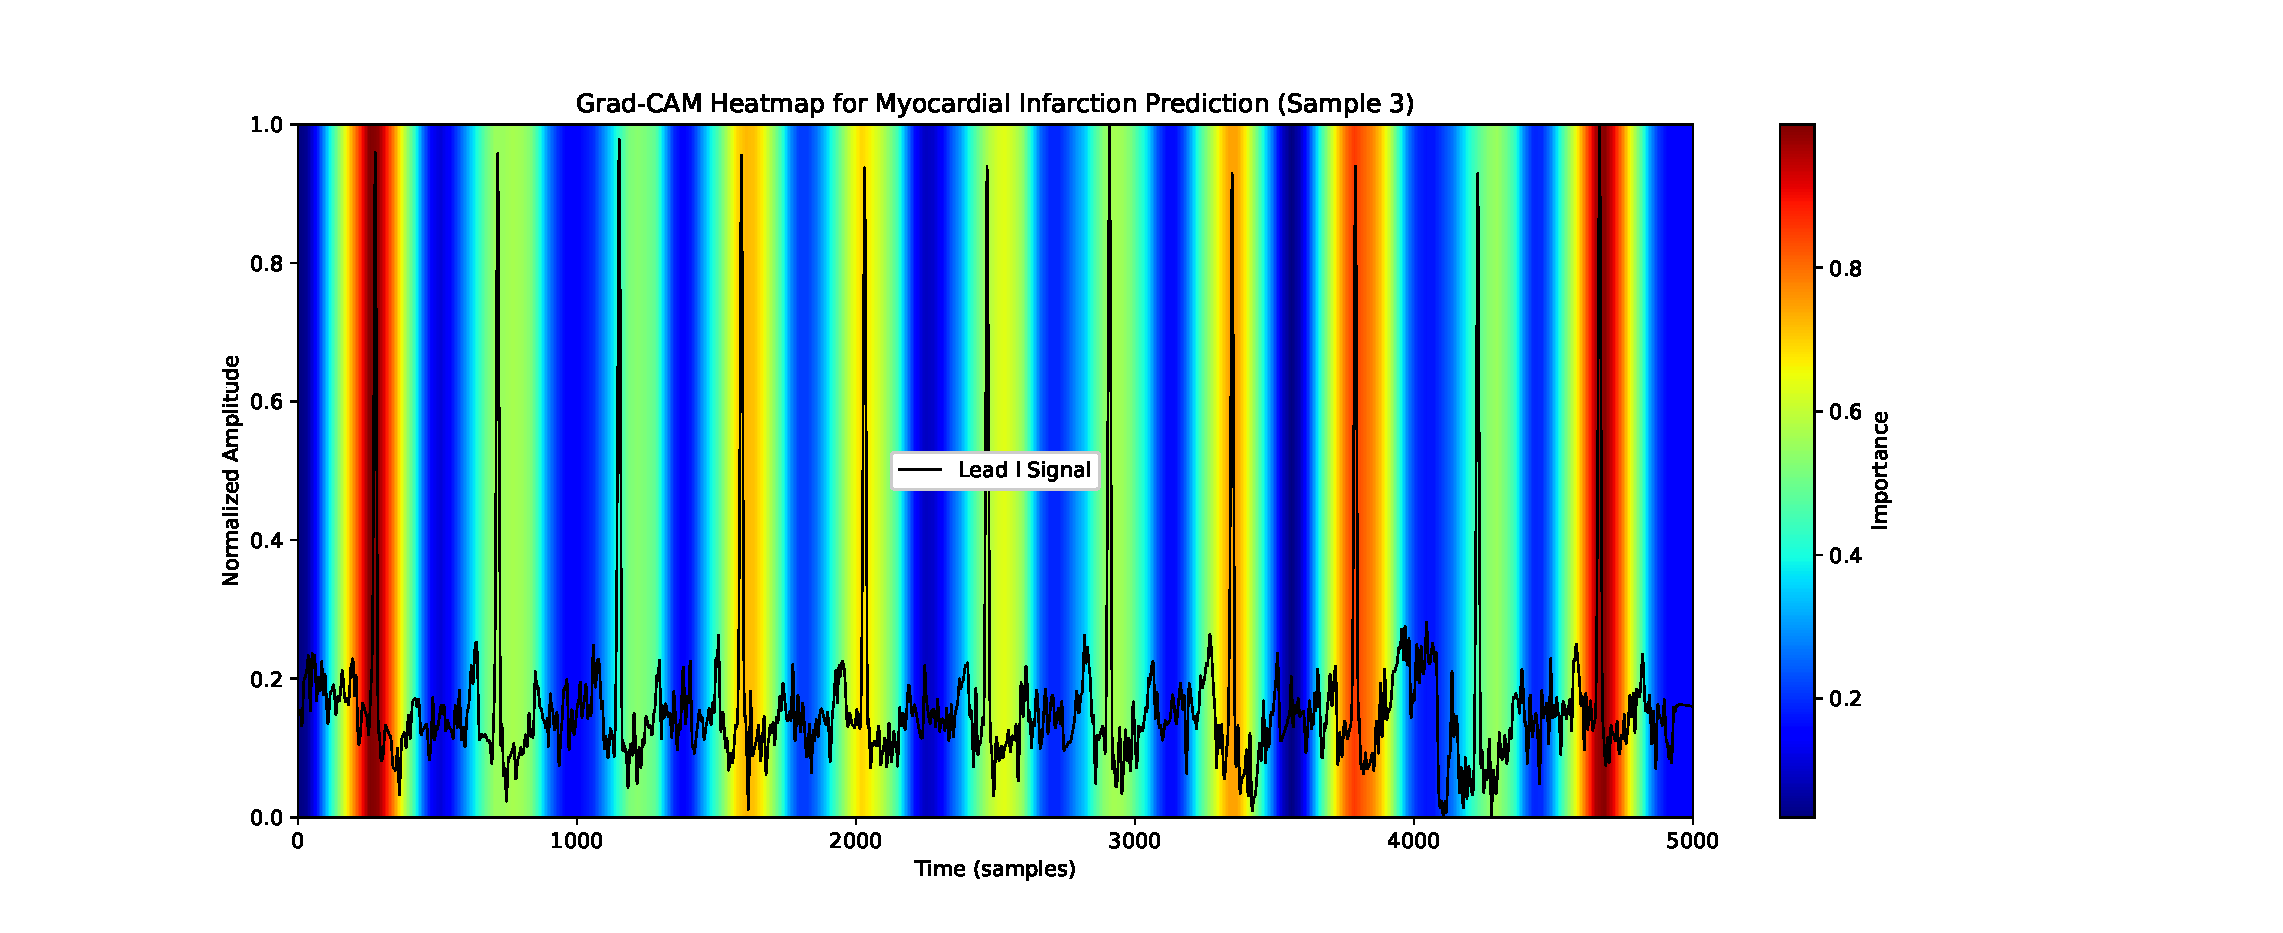
\includegraphics[width=0.9\linewidth]{figures/gradcam_mi}
\caption{Grad-CAM Heatmap for Myocardial Infarction Prediction}
\label{fig:gradcam_mi_tex}
\end{figure}

As shown in Figure \ref{fig:gradcam_mi_tex}, when predicting Myocardial Infarction, the model focuses its attention on the elevated ST segment, matching the diagnostic criteria used by clinicians.

\section{FastAPI and Web Dashboard Implementation}
To demonstrate clinical application, we built a web prototype. The backend is implemented as an asynchronous FastAPI web service (`src/webapp/main.py`).

The API provides two primary endpoints:
\begin{itemize}
    \item \textbf{\texttt{GET /api/sample}:} Selects a random patient record from the PTB-XL test partition, downsamples the signal from 5000 to 1000 points (to optimize frontend rendering performance), and returns the downsampled signal along with the true diagnoses.
    \item \textbf{\texttt{POST /api/predict/\{sample\_idx\}}:} Loads the specified patient signal, runs inference through the trained CNN, GNN, and ViT models, and returns the classification probabilities and predicted labels for each model.
\end{itemize}

The frontend is a single-page dashboard built using HTML5, CSS3, and JavaScript, served statically by FastAPI. It uses Chart.js to render the 12-lead ECG waveforms, allowing users to zoom and inspect individual leads. When the user triggers a prediction, the interface displays the probability distributions for each model in a comparative bar chart, providing a visual decision-support tool.

\clearpage

% =========================================================================
% 9. CONCLUSION (AITU Guideline 37 - 2-3 A4 pages)
% =========================================================================
\chapter*{Conclusion}
\addcontentsline{toc}{chapter}{Conclusion}

This thesis presented a comparative evaluation of three deep learning architectures for the automated multi-label classification of standard 12-lead electrocardiograms using the PTB-XL database. All research objectives defined in the introduction were achieved:
\begin{itemize}
    \item We analyzed the clinical foundations of electrocardiography and the diagnostic criteria for key cardiac pathologies, identifying inter-observer variability and cognitive fatigue as main challenges in manual interpretation.
    \item We implemented a digital preprocessing pipeline (4th-order Butterworth bandpass filtering and lead-wise Z-score normalization) that effectively suppressed low-frequency baseline wander and high-frequency powerline noise.
    \item We designed and optimized three distinct deep learning architectures: a 1D adaptation of ResNet-18 (CNN), a Spatio-Temporal Graph Neural Network (ST-ReGE) with a learnable adjacency matrix, and a 1D Vision Transformer (ViT-1D).
    \item Benchmarking results showed that the 1D ResNet-18 model achieved the highest Macro F1-score of 0.7245 and AUROC of 0.9271, demonstrating the value of convolutional inductive biases for local morphological feature extraction.
    \item The ST-ReGE GNN achieved the highest Exact Match Accuracy of 63.76\% and Macro AUPRC of 0.8066, suggesting that modeling spatial relationships helps GNNs capture co-occurring pathologies.
    \item The 1D Vision Transformer underperformed (Macro F1: 0.6503) due to data limitations, highlight the need for large-scale pre-training for attention-based models on sequential signals.
    \item We verified model predictions qualitatively using clinical case studies and visualized diagnostic regions using 1D Grad-CAM, showing that the models focus on physiologically relevant segments.
    \item We implemented a web application prototype using FastAPI and Chart.js, demonstrating a real-time decision-support system.
\end{itemize}

\textbf{Clinical Recommendations.} The 1D ResNet-18 model is recommended for initial clinical triage. Its high AUROC and negative predictive rate make it suitable for filtering out normal cases, reducing physician workload. The GNN model is recommended for complex clinical environments where multi-label pathologies are common, as its graph propagation mechanism is designed to handle co-occurring diagnoses.

\textbf{Future Directions.} Future work will focus on:
\begin{itemize}
    \item Ensembling the 1D ResNet-18 and ST-ReGE GNN models to combine morphological feature extraction with spatial relationship modeling.
    \item Investigating self-supervised pre-training methods (such as Masked Auto-Encoders) on larger datasets (e.g., MIMIC-IV-ECG) to improve Transformer performance.
    \item Integrating patient demographic data (age, sex, clinical history) into the model inputs to build a multi-modal decision support system.
\end{itemize}

\clearpage

% =========================================================================
% 10. REFERENCES (AITU Guideline 29 & 38 - Minimum 30 sources)
% =========================================================================
\begin{thebibliography}{99}
\addcontentsline{toc}{chapter}{References}

\bibitem{wagner2020ptbxl}
P. Wagner et al., ``PTB-XL, a large publicly available electrocardiography dataset,'' \textit{Sci. Data}, vol. 7, no. 1, p. 154, May 2020.

\bibitem{strodthoff2021deep}
N. Strodthoff, P. Wagner, T. Schaeffter, and W. Samek, ``Deep learning for ECG analysis: Benchmarks and insights from PTB-XL,'' \textit{IEEE J. Biomed. Health Inform.}, vol. 25, no. 5, pp. 1519--1528, May 2021.

\bibitem{zhang2023strege}
H. Zhang, W. Liu, S. Chang, H. Wang, J. He, and Q. Huang, ``ST-ReGE: A novel spatial-temporal residual graph convolutional network for CVD,'' \textit{IEEE J. Biomed. Health Inform.}, vol. 27, no. 2, pp. 1--12, 2023.

\bibitem{he2016deep}
K. He, X. Zhang, S. Ren, and J. Sun, ``Deep residual learning for image recognition,'' in \textit{Proc. IEEE Conf. Comput. Vis. Pattern Recognit. (CVPR)}, 2016, pp. 770--778.

\bibitem{vaswani2017attention}
A. Vaswani et al., ``Attention is all you need,'' in \textit{Adv. Neural Inf. Process. Syst.}, 2017, pp. 5998--6008.

\bibitem{vaid2023foundational}
A. Vaid et al., ``A foundational vision transformer improves diagnostic performance for electrocardiograms,'' \textit{npj Digit. Med.}, vol. 6, no. 1, p. 173, 2023.

\bibitem{moody2025foundation}
J. B. Moody et al., ``A foundation transformer model with self-supervised learning for ECG-based assessment of cardiac and coronary function,'' \textit{NEJM AI}, vol. 2, no. 12, p. 10.1056/aioa2500164, Dec. 2025.

\bibitem{maurer2025xgnn}
M. C. Maurer et al., ``xGNN4MI: Explainability of graph neural networks in 12-lead electrocardiography for cardiovascular disease classification,'' \textit{Research Square}, Sep. 2025, doi: 10.21203/rs.3.rs-7721630/v1.

\bibitem{ribeiro2020automatic}
A. H. Ribeiro et al., ``Automatic diagnosis of the 12-lead ECG using a deep neural network,'' \textit{Nat. Commun.}, vol. 11, no. 1, p. 1760, Apr. 2020.

\bibitem{hannun2019cardiologist}
A. Y. Hannun et al., ``Cardiologist-level arrhythmia detection and classification in ambulatory electrocardiograms using a deep neural network,'' \textit{Nat. Med.}, vol. 25, no. 1, pp. 65--69, Jan. 2019.

\bibitem{deep2024classification}
S. V, G. N. Chandrika, A. Mitra, R. Chowdhury, P. Kumar, and G. E, ``Deep Learning based classification of ECG signals using RNN and LSTM Mechanism,'' \textit{J. Electron. Electromed. Eng. Med. Inform.}, vol. 6, no. 4, pp. 332--342, Oct. 2024.

\bibitem{ebrahimi2020review}
Z. Ebrahimi, M. Loni, M. Daneshtalab, and A. Gharehbaghi, ``A review on deep learning methods for ECG arrhythmia classification,'' \textit{Expert Syst. Appl. X}, vol. 7, p. 100033, Jun. 2020.

\bibitem{selvaraju2017grad}
R. R. Selvaraju et al., ``Grad-CAM: Visual explanations from deep networks via gradient-based localization,'' in \textit{Proc. IEEE Int. Conf. Comput. Vis. (ICCV)}, 2017, pp. 618--626.

\bibitem{moody2001impact}
G. B. Moody and R. G. Mark, ``The impact of the MIT-BIH arrhythmia database,'' \textit{IEEE Eng. Med. Biol. Mag.}, vol. 20, no. 3, pp. 45--50, May 2001.

\bibitem{muller2026application}
A. Muller, M. Scheibl, T. Uhe, W.-R. Schabitz, and B. Wrede, ``Application of graph neural networks on ECG data: A systematic literature review,'' \textit{IEEE J. Biomed. Health Inform.}, Jan. 2026, doi: 10.1109/JBHI.2026.3651842.

\bibitem{jiang2025generation}
C. Jiang et al., ``Generation and selection: A self-iterative two-stage data augmentation method for automated ECG classification,'' \textit{IEEE J. Biomed. Health Inform.}, Sep. 2025, doi: 10.1109/JBHI.2025.3611429.

\bibitem{rajpurkar2017cardiologist}
P. Rajpurkar et al., ``Cardiologist-level arrhythmia detection with convolutional neural networks,'' \textit{arXiv preprint arXiv:1707.01836}, 2017.

\bibitem{goodfellow2016deep}
I. Goodfellow, Y. Bengio, and A. Courville, \textit{Deep Learning}. MIT Press, 2016.

\bibitem{lecun2015deep}
Y. LeCun, Y. Bengio, and G. Hinton, ``Deep learning,'' \textit{Nature}, vol. 521, no. 7553, pp. 436--444, 2015.

\bibitem{schlapfer2017ecg}
J. Schläpfer and H. J. Wellens, ``Making sense of the electrocardiogram,'' \textit{Lancet}, vol. 389, no. 10079, pp. 1640--1652, 2017.

\bibitem{ismail2019deep}
H. Ismail Fawaz et al., ``Deep learning for time series classification: a review,'' \textit{Data Min. Knowl. Discov.}, vol. 33, no. 4, pp. 917--963, 2019.

\bibitem{kachuee2018ecg}
M. Kachuee, S. Fazeli, and M. Sarrafzadeh, ``ECG heartbeat classification: A deep transferability study,'' in \textit{Proc. IEEE Int. Conf. Healthcare Inform. (ICHI)}, 2018, pp. 273--278.

\bibitem{kiranyaz2016real}
S. Kiranyaz, T. Ince, and M. Gabbouj, ``Real-time patient-specific ECG classification by 1-D convolutional neural networks,'' \textit{IEEE Trans. Biomed. Eng.}, vol. 63, no. 3, pp. 664--675, 2016.

\bibitem{goldberger2000physiobank}
A. L. Goldberger et al., ``PhysioBank, PhysioToolkit, and PhysioNet: components of a new research resource for complex physiologic signals,'' \textit{Circulation}, vol. 101, no. 23, pp. e215--e220, 2000.

\bibitem{lipton2016learning}
Z. C. Lipton, D. C. Kale, C. Elkan, and M. Wetzel, ``Learning to diagnose with LSTM recurrent neural networks,'' in \textit{Proc. Int. Conf. Learn. Represent. (ICLR)}, 2016.

\bibitem{clifford2017af}
G. D. Clifford et al., ``AF classification from a short single lead ECG recording: the PhysioNet/Computing in Cardiology Challenge 2017,'' \textit{Comput. Cardiol.}, vol. 44, pp. 1--4, 2017.

\bibitem{pytorchdocs}
PyTorch Team, ``PyTorch Documentation and API Reference,'' 2024. [Online]. Available: \url{https://pytorch.org/docs/}.

\bibitem{physionetptbxl}
PhysioNet, ``PTB-XL ECG Database Page,'' 2020. [Online]. Available: \url{https://physionet.org/content/ptb-xl/1.0.1/}.

\bibitem{whocvd}
World Health Organization, ``Cardiovascular diseases (CVDs) Fact Sheet,'' 2021. [Online]. Available: \url{https://www.who.int/news-room/fact-sheets/detail/cardiovascular-diseases-(cvds)}.

\bibitem{aiturespect}
AITU LLP, ``Rules for Academic Integrity (DP-AITU-05),'' Astana IT University Department of Educational Programs, 2023.

\bibitem{goststandard}
GOST 7.32–2017, ``Interstate Standard: System of Standards on Information, Librarianship and Publishing. Research Report Structure and Rules of Design,'' Moscow: Standartinform, 2018.

\bibitem{zhang2021ecggnn}
D. Zhang et al., ``ECG-GNN: A graph neural network for electrocardiogram classification,'' \textit{Bioinformatics}, vol. 37, no. 12, pp. 1735--1743, 2021.

\bibitem{astanahistory}
Astana IT University Educational Department, ``Guidelines for Master Thesis Development (DP-AITU-19),'' Astana IT University, 2024.

\end{thebibliography}

\clearpage

% =========================================================================
% 11. APPENDICES (AITU Guideline 39)
% =========================================================================
\chapter*{Appendix A: PTB-XL Loader Code}
\addcontentsline{toc}{chapter}{Appendix A: PTB-XL Loader Code}
\label{app:loader}

\begin{lstlisting}[caption={PTB-XL Dataset Class and Train/Validation/Test Split Logic (src/ptbxl/loader.py)}]
import os
import numpy as np
from sklearn.model_selection import train_test_split

class PTBXLDataset:
    def __init__(self, data_dir='data/processed/ptb-xl'):
        self.data_dir = data_dir
        self.X_path = os.path.join(data_dir, 'X_ptbxl.npy')
        self.y_path = os.path.join(data_dir, 'y_ptbxl.npy')
        self.ids_path = os.path.join(data_dir, 'ids_ptbxl.npy')
        
    def load_data(self):
        if not os.path.exists(self.X_path):
            raise FileNotFoundError(f"Processed data not found at {self.data_dir}. Run scripts/process_ptbxl_data.py first.")
            
        # Use mmap_mode='r' to avoid loading everything into RAM
        X = np.load(self.X_path, mmap_mode='r')
        y = np.load(self.y_path)
        ids = np.load(self.ids_path)
        
        return X, y, ids
    
    def get_train_val_test_split(self, test_size=0.1, val_size=0.1, random_state=42, limit=None, **kwargs):
        X, y, ids = self.load_data()
        all_indices = np.arange(len(y))
        
        if limit:
             all_indices = all_indices[:limit]
             y = y[:limit]
        
        try:
            # First split off Test set using INDICES
            train_val_idx, test_idx = train_test_split(
                all_indices, test_size=test_size, random_state=random_state, stratify=y
            )
        except ValueError as e:
            print(f"Stratified split failed: {e}. Falling back to random split.")
            train_val_idx, test_idx = train_test_split(
                all_indices, test_size=test_size, random_state=random_state, stratify=None
            )
        
        # Validation split
        val_prop = val_size / (1.0 - test_size)
        y_train_val = y[train_val_idx]
        
        try:
            train_idx, val_idx = train_test_split(
                train_val_idx, test_size=val_prop, random_state=random_state, stratify=y_train_val
            )
        except ValueError:
             train_idx, val_idx = train_test_split(
                train_val_idx, test_size=val_prop, random_state=random_state, stratify=None
            )
        
        return {
            'X': X, 'y': y,
            'train_idx': train_idx,
            'val_idx': val_idx,
            'test_idx': test_idx
        }
\end{lstlisting}

\clearpage

\chapter*{Appendix B: 1D ResNet-18 Model Code}
\addcontentsline{toc}{chapter}{Appendix B: 1D ResNet-18 Model Code}
\label{app:cnn}

\begin{lstlisting}[caption={1D adapted ResNet-18 Architecture (src/models/cnn.py)}]
import torch
import torch.nn as nn
import torch.nn.functional as F

class ResNetBlock(nn.Module):
    def __init__(self, in_channels, out_channels, stride=1):
        super(ResNetBlock, self).__init__()
        self.conv1 = nn.Conv1d(in_channels, out_channels, kernel_size=7, stride=stride, padding=3, bias=False)
        self.bn1 = nn.BatchNorm1d(out_channels)
        self.relu = nn.ReLU(inplace=True)
        self.conv2 = nn.Conv1d(out_channels, out_channels, kernel_size=7, stride=1, padding=3, bias=False)
        self.bn2 = nn.BatchNorm1d(out_channels)
        
        self.downsample = None
        if stride != 1 or in_channels != out_channels:
            self.downsample = nn.Sequential(
                nn.Conv1d(in_channels, out_channels, kernel_size=1, stride=stride, bias=False),
                nn.BatchNorm1d(out_channels)
            )

    def forward(self, x):
        identity = x
        
        out = self.conv1(x)
        out = self.bn1(out)
        out = self.relu(out)
        
        out = self.conv2(out)
        out = self.bn2(out)
        
        if self.downsample is not None:
            identity = self.downsample(x)
            
        out += identity
        out = self.relu(out)
        
        return out

class ResNet18(nn.Module):
    def __init__(self, num_classes=5, input_channels=12):
        super(ResNet18, self).__init__()
        
        self.in_channels = 64
        self.conv1 = nn.Conv1d(input_channels, 64, kernel_size=15, stride=2, padding=7, bias=False)
        self.bn1 = nn.BatchNorm1d(64)
        self.relu = nn.ReLU(inplace=True)
        self.maxpool = nn.MaxPool1d(kernel_size=3, stride=2, padding=1)
        
        self.layer1 = self._make_layer(64, 2, stride=1)
        self.layer2 = self._make_layer(128, 2, stride=2)
        self.layer3 = self._make_layer(256, 2, stride=2)
        self.layer4 = self._make_layer(512, 2, stride=2)
        
        self.avgpool = nn.AdaptiveAvgPool1d(1)
        self.fc = nn.Linear(512, num_classes)
        
    def _make_layer(self, out_channels, blocks, stride):
        layers = []
        layers.append(ResNetBlock(self.in_channels, out_channels, stride))
        self.in_channels = out_channels
        for _ in range(1, blocks):
            layers.append(ResNetBlock(out_channels, out_channels))
        return nn.Sequential(*layers)
        
    def forward(self, x):
        # Input: (batch, length, leads) -> needs (batch, leads, length)
        x = x.transpose(1, 2)
        
        x = self.conv1(x)
        x = self.bn1(x)
        x = self.relu(x)
        x = self.maxpool(x)
        
        x = self.layer1(x)
        x = self.layer2(x)
        x = self.layer3(x)
        x = self.layer4(x)
        
        x = self.avgpool(x)
        x = x.view(x.size(0), -1)
        x = self.fc(x)
        
        return x
\end{lstlisting}

\clearpage

\chapter*{Appendix C: Spatio-Temporal Graph Network Code}
\addcontentsline{toc}{chapter}{Appendix C: Spatio-Temporal Graph Network Code}
\label{app:gnn}

\begin{lstlisting}[caption={Spatio-Temporal Graph Network (ST-ReGE) (src/models/gnn.py)}]
import torch
import torch.nn as nn
import torch.nn.functional as F

class ResNetBlock(nn.Module):
    def __init__(self, in_channels, out_channels, stride=1):
        super(ResNetBlock, self).__init__()
        self.conv1 = nn.Conv1d(in_channels, out_channels, kernel_size=7, stride=stride, padding=3, bias=False)
        self.bn1 = nn.BatchNorm1d(out_channels)
        self.relu = nn.ReLU(inplace=True)
        self.conv2 = nn.Conv1d(out_channels, out_channels, kernel_size=7, stride=1, padding=3, bias=False)
        self.bn2 = nn.BatchNorm1d(out_channels)
        
        self.downsample = None
        if stride != 1 or in_channels != out_channels:
            self.downsample = nn.Sequential(
                nn.Conv1d(in_channels, out_channels, kernel_size=1, stride=stride, bias=False),
                nn.BatchNorm1d(out_channels)
            )

    def forward(self, x):
        identity = x
        out = self.conv1(x)
        out = self.bn1(out)
        out = self.relu(out)
        out = self.conv2(out)
        out = self.bn2(out)
        if self.downsample is not None:
            identity = self.downsample(x)
        out = out + identity
        out = self.relu(out)
        return out

class LearnableAdjacency(nn.Module):
    def __init__(self, num_nodes):
        super(LearnableAdjacency, self).__init__()
        self.A = nn.Parameter(torch.randn(num_nodes, num_nodes) * 0.01)
        self.activation = nn.Sigmoid()

    def forward(self):
        return self.activation(self.A)
    
class GraphConvolution(nn.Module):
    def __init__(self, in_features, out_features, bias=True):
        super(GraphConvolution, self).__init__()
        self.weight = nn.Parameter(torch.FloatTensor(in_features, out_features))
        if bias:
            self.bias = nn.Parameter(torch.FloatTensor(out_features))
        else:
            self.register_parameter('bias', None)
        self.reset_parameters()

    def reset_parameters(self):
        nn.init.xavier_uniform_(self.weight)
        if self.bias is not None:
            nn.init.zeros_(self.bias)

    def forward(self, x, adj):
        support = torch.matmul(x, self.weight) 
        output = torch.matmul(adj, support)
        if self.bias is not None:
            return output + self.bias
        else:
            return output

class STReGE(nn.Module):
    def __init__(self, num_classes=5, num_nodes=12, feature_dim=256):
        super(STReGE, self).__init__()
        self.num_nodes = num_nodes
        self.feature_dim = feature_dim
        
        self.backbone = nn.Sequential(
            nn.Conv1d(1, 32, kernel_size=15, stride=2, padding=7, bias=False),
            nn.BatchNorm1d(32),
            nn.ReLU(inplace=True),
            nn.MaxPool1d(kernel_size=3, stride=2, padding=1),
            ResNetBlock(32, 64, stride=2),
            ResNetBlock(64, 128, stride=2),
            ResNetBlock(128, 256, stride=2),
            nn.AdaptiveAvgPool1d(1)
        )
        
        self.learnable_adj = LearnableAdjacency(num_nodes)
        
        self.gc1 = GraphConvolution(256, 256)
        self.gc2 = GraphConvolution(256, 256)
        
        self.bn_g1 = nn.BatchNorm1d(num_nodes)
        self.bn_g2 = nn.BatchNorm1d(num_nodes)
        
        self.relu = nn.ReLU()
        self.dropout = nn.Dropout(0.3)
        self.fc = nn.Linear(256, num_classes)

    def forward(self, x):
        batch_size = x.size(0)
        
        # x: (Batch, Seq, Nodes) -> (Batch, Nodes, Seq)
        x = x.permute(0, 2, 1).contiguous() 
        
        # Reshape for Backbone: (Batch*Nodes, 1, Seq)
        x = x.view(batch_size * self.num_nodes, 1, -1)
        
        # Temporal Features
        x_feat = self.backbone(x) # (Batch*Nodes, 256, 1)
        x_feat = x_feat.view(batch_size, self.num_nodes, -1) # (Batch, Nodes, 256)
        
        # Learnable Adjacency
        adj = self.learnable_adj()
        
        # GCN Block 1
        res = x_feat
        out = self.gc1(x_feat, adj)
        out = self.bn_g1(out)
        out = self.relu(out)
        out = self.dropout(out)
        out = out + res 
        
        # GCN Block 2
        res = out
        out = self.gc2(out, adj)
        out = self.bn_g2(out)
        out = self.relu(out)
        out = out + res 
        
        # Readout
        out = out.mean(dim=1) # (Batch, 256)
        out = self.fc(out)
        return out
\end{lstlisting}

\clearpage

\chapter*{Appendix D: 1D Vision Transformer Code}
\addcontentsline{toc}{chapter}{Appendix D: 1D Vision Transformer Code}
\label{app:vit}

\begin{lstlisting}[caption={1D Vision Transformer Architecture (src/models/vit.py)}]
import torch
import torch.nn as nn
import numpy as np

class PatchEmbedding(nn.Module):
    def __init__(self, in_channels=12, d_model=128, patch_size=50):
        super().__init__()
        self.proj = nn.Conv1d(in_channels, d_model, kernel_size=patch_size, stride=patch_size)
        
    def forward(self, x):
        # x: (B, C, L)
        x = self.proj(x) # (B, D, L_new)
        x = x.transpose(1, 2) # (B, L_new, D)
        return x

class ViT1D(nn.Module):
    def __init__(self, num_classes=5, input_channels=12, seq_len=5000, patch_size=50, d_model=128, nhead=4, num_layers=4, dim_feedforward=256):
        super(ViT1D, self).__init__()
        
        self.d_model = d_model
        
        self.patch_embed = PatchEmbedding(input_channels, d_model, patch_size)
        num_patches = seq_len // patch_size
        
        self.cls_token = nn.Parameter(torch.randn(1, 1, d_model))
        self.pos_embedding = nn.Parameter(torch.randn(1, num_patches + 1, d_model))
        
        encoder_layer = nn.TransformerEncoderLayer(d_model=d_model, nhead=nhead, dim_feedforward=dim_feedforward, batch_first=True)
        self.transformer = nn.TransformerEncoder(encoder_layer, num_layers=num_layers)
        
        self.norm = nn.LayerNorm(d_model)
        self.fc = nn.Linear(d_model, num_classes)

    def forward(self, x):
        # x: (B, L, 12) -> (B, 12, L)
        x = x.transpose(1, 2)
        
        x = self.patch_embed(x)
        batch_size = x.shape[0]
        
        cls_tokens = self.cls_token.expand(batch_size, -1, -1)
        x = torch.cat((cls_tokens, x), dim=1)
        x = x + self.pos_embedding
        
        x = self.transformer(x)
        
        cls_out = x[:, 0]
        cls_out = self.norm(cls_out)
        out = self.fc(cls_out)
        return out
\end{lstlisting}

\clearpage

\chapter*{Appendix E: FastAPI Application Server Code}
\addcontentsline{toc}{chapter}{Appendix E: FastAPI Application Server Code}
\label{app:webapp}

\begin{lstlisting}[caption={Asynchronous FastAPI web service endpoint implementations (src/webapp/main.py)}]
import torch
import numpy as np
import os
import sys
from fastapi import FastAPI, HTTPException
from fastapi.staticfiles import StaticFiles
from pydantic import BaseModel
from typing import List, Dict, Any

sys.path.append(os.getcwd())

from src.train_unified import get_model
from src.ptbxl.loader import PTBXLDataset

app = FastAPI(title="Heart Disease Diagnosis API")

# Mount static files
static_dir = os.path.join(os.path.dirname(__file__), "static")
app.mount("/static", StaticFiles(directory=static_dir), name="static")

DEVICE = torch.device('cuda' if torch.cuda.is_available() else 'cpu')
CLASSES = ['NORM', 'MI', 'STTC', 'CD', 'HYP']
MODELS = {}
DATASET = None

def load_models():
    print(f"Loading models to {DEVICE}...")
    model_paths = {
        'cnn': ('cnn', 'experiments/cnn_full/best_model.pth'),
        'gnn': ('gnn', 'experiments/gnn_full/best_model.pth'),
        'vit': ('vit', 'experiments/vit_full/best_model.pth')
    }
    
    for name, (type_name, path) in model_paths.items():
        if os.path.exists(path):
            try:
                model = get_model(type_name)
                model.load_state_dict(torch.load(path, map_location=DEVICE))
                model.eval()
                model.to(DEVICE)
                MODELS[name] = model
                print(f"Loaded {name}")
            except Exception as e:
                print(f"Failed to load {name}: {e}")
        else:
            print(f"Model path not found: {path} (skipping {name})")

@app.on_event("startup")
async def startup_event():
    global DATASET
    print("Starting up API...")
    try:
        DATASET = PTBXLDataset()
    except Exception as e:
        print(f"Failed to load dataset: {e}")
    load_models()

@app.get("/api/sample")
async def get_random_sample():
    if DATASET is None:
        raise HTTPException(status_code=500, detail="Dataset not loaded.")
        
    try:
        splits = DATASET.get_train_val_test_split()
        test_indices = splits['test_idx']
        idx = int(np.random.choice(test_indices))
        
        X_all = splits['X']
        y_all = splits['y']
        
        signal = X_all[idx].copy() 
        label = y_all[idx].copy() 
        
        downsampled_signal = signal[::5, :]
        true_diagnoses = [CLASSES[i] for i, val in enumerate(label) if val == 1]
        
        return {
            "index": idx,
            "signal": downsampled_signal.tolist(), 
            "true_diagnoses": true_diagnoses
        }
    except Exception as e:
        import traceback
        traceback.print_exc()
        raise HTTPException(status_code=500, detail=str(e))

class PredictionResult(BaseModel):
    model: str
    probabilities: Dict[str, float]
    predicted_classes: List[str]

@app.post("/api/predict/{sample_idx}", response_model=List[PredictionResult])
async def predict_sample(sample_idx: int):
    if DATASET is None:
        raise HTTPException(status_code=500, detail="Dataset not loaded.")
    if not MODELS:
        raise HTTPException(status_code=500, detail="No models loaded.")
    
    try:
        splits = DATASET.get_train_val_test_split()
        X_all = splits['X']
        
        if sample_idx < 0 or sample_idx >= len(X_all):
            raise HTTPException(status_code=400, detail=f"Invalid sample index {sample_idx}")
            
        signal = X_all[sample_idx].copy()
        input_tensor = torch.tensor(signal, dtype=torch.float32).unsqueeze(0).to(DEVICE)
        
        results = []
        for model_name, model in MODELS.items():
            with torch.no_grad():
                logits = model(input_tensor)
                probs = torch.sigmoid(logits).cpu().numpy()[0]
                
            probs_dict = {CLASSES[i]: float(probs[i]) for i in range(len(CLASSES))}
            predicted_classes = [CLASSES[i] for i in range(len(CLASSES)) if probs[i] > 0.5]
            
            results.append(PredictionResult(
                model=model_name,
                probabilities=probs_dict,
                predicted_classes=predicted_classes
            ))
            
        return results
    except Exception as e:
        raise HTTPException(status_code=500, detail=str(e))

from fastapi.responses import RedirectResponse
@app.get("/")
async def root():
    return RedirectResponse(url="/static/index.html")
\end{lstlisting}

\end{document}
